\section{PAC Learning}



\subsection{The PAC Learning Model}
\textbf{$\epsilon$ error parameter, $\delta$ confidence val}
\begin{itemize}
	\item PAC learn.: $
			\P(\mathcal R(\hat{c}_n^*)$ $\leq$ $\epsilon)$ $\geq$ $1 -\delta
		$
		
		\item General Setting: 
		$
			\P(\mathcal R(\hat{c}_n^*) - \inf_{c\in \mathcal C} \mathcal R(c) \leq \epsilon) \geq 1 - \delta
		$
	\item Efficiently PAC learnable: Algorithm runs in poly time in $1/\epsilon$ and $1/\delta$ (computing $X_{\textit{min}}^n$ and compl. of $n$)
\end{itemize}






\subsection{Rectangle Learning}
Pick tight rectangle. Diff between picked rectangle $\hat R$ and true rectangle $R$ with few examples. Rectangles are efficiently PAC learnable.


\subsection{Example: Half-line learning}
$\mathcal C = \mathcal H = \{\mathbb I_{[l, \infty)} : l\in \mathbb R\}$, where 
\begin{minipage}{\columnwidth}
	\begin{minipage}{0.5\columnwidth}
		$\mathbb I_{[l, \infty)} = 
		\begin{cases}
			0 & x < l \\
			1 & x \geq l
		\end{cases}
		$
	\end{minipage}
	\begin{minipage}{0.45\columnwidth}
		\textit{fix $f^*\in \mathbb R$, consider $c^* = \mathbb I_{[l^*, \infty)}$}
	\end{minipage}
\end{minipage}

let $X_{\textit{min}}^n := \min_{i\leq n, Y_i=1} X_i, \hat c_n := \mathbb I_{X_{\textit{min}}^n}, \infty)$


Let $l_\epsilon^+\in\R$ s.t. $\P(l^*\leq X_i \leq l_\epsilon^+) = \epsilon$.
\begin{center}
	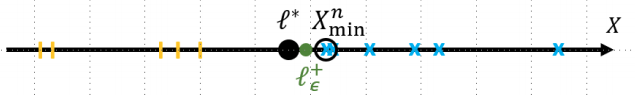
\includegraphics[width=\columnwidth]{Resources/pac-halfline}
\end{center}
If $l_\epsilon^+ \leq X_{\textit{min}}^n$: $l^*\leq X_i \leq X_{\textit{min}}^n$.

Then $\mathcal R(\hat c_n) = \P(l^*\leq X_i \leq X_{\textit{min}}^n)$ ${\color{imp}\geq} \P(l^*\leq X_i \leq l_\epsilon^+) = \epsilon$

$\P(l_\epsilon^+\leq X_{\textit{min}}^n) = \prod_i^n \P[X_i\not\in[l^*, l_\epsilon^+)] = \prod(1 - \P(l^*\leq X_i \leq l_\epsilon^+)) = (1-\epsilon)^n$

$\P(\mathcal R(\hat c_n)\geq \epsilon) = \P(l_\epsilon^+\leq X_{\textit{min}}^n)$ 
$= (1-\epsilon)^n {\color{imp} \leq \delta}$. $\to n \geq \frac{1}{\epsilon}\log\frac{1}{\delta}$.

%\subsubsection{The general PAC model}
%A learning algorithm $\mathcal A$ can learn a concept class $\mathcal C$ from $\mathcal H$ if given {\color{imp3}sufficiently large sample} as input, outputs a hypothesis that \textbf{{\color{imp}generalizes well} {\color{imp2}with high probability}}
%
%\textbf{Definition: } A learning algorithm $\mathcal A$ can learn a concept class $\mathcal C$ from $\mathcal H$ if there is a {\color{imp3} polynomial function $\mathit{poly}$}, such that
%\begin{enumerate}
%	\item For any distribution $\mathcal D$ on $\mathcal X\times \{0,1\}$ and
%	\item for any {\color{imp}$0<\epsilon<1/2$} and {\color{imp2}$0<\delta<1/2$}
%\end{enumerate}
%if $\mathcal A$ receives as input {\color{imp3} a sample $\mathcal Z$ of size $n\geq \mathit{poly}(1/\epsilon, 1/\delta, \mathit{dim}(\mathcal X)$}, then $\mathcal A$ outputs $\hat c\in\mathcal H$, sucht that
%$
%	{\color{imp2}\P_{\mathcal Z\sim \mathcal D^n}\left({\color{imp}\mathcal R(\hat c) - \inf_{c\in\mathcal C}\mathcal R(c)\leq \epsilon }\right) \geq 1 - \delta}
%$
%
